\section{Workflow}
As illustrated in the left of Figure \ref{fig:teaser}, our workflow starts from physically collecting branches.
The collected branches are uploaded to cloud database by \textit{Branch Importer}, and served to the online game-based design application \textit{BranchConnect}.
The game system uses skeletons for its joint detection process working on browsers and accessible from laptop computers and mobile devices.
As in the right of \ref{fig:teaser}, users can explore a global design with multiple branch layouts.
Once the global design is fixed, designed layouts are further inspected by \textit{G-Code Generator}, which generates customized joineries for CNC milling.
After finishing the milling process, users physically assemble branches and complete the fabrication process.
The pipeline of the workflow is illustrated in the Figure \ref{fig:pipeline}.
In this section, we introduce two steps in the pipeline: Digital Model Acquisition and Fabrication.
As for the game system, please refer Section \ref{sec:game}.

\begin{figure}[ht]
  \begin{center}
    \includegraphics[width = 0.4\paperwidth]{images/workflow/pipeline.png}
    \caption{A pipeline from model acquisition to fabrication.}
    \label{fig:pipeline}
  \end{center}
\end{figure}

\subsection{Digital Model Acquisition}
Our system takes textured mesh model or point cloud with colored vertices.
As complete mesh model provides more robust results with 3D shapes of branches, we describe our process based on mesh model as an input.
There are various methods and software available for scanning 3D models.
As for scanning setup, we describe in the Section \ref{sec:casestudy}.
Taking mesh model with colored texture, our \textit{Branch Importer} provides functions such as object detection, skeleton extraction, branch type classification, and fixture point setting.

The scanned result is a mesh model representing branches with a fixed plate.
The system first idendifies branches by applying simple height threshold, and then applies contour detection (we currently use \textit{findContour} in OpenCV \footnote{Open Source Computer Vision Library: \url{http://opencv.org/} }).
The obtained 2D contours are used for extracting skeletons and clustering point cloud in the mesh model.
Contours are triangulated and skeleton points are extracted from middle points on edges of triangles.
These middle points are compared with top view image from OpenCV.
If the point is inside of a contour, the middle point is counted as a valid point.
After extracting valid middle points, the connectivity of skeletons is analyzed.
In case grafting branch is detected, a new skeleton sub-branch is added.
The result is shown in Figure ~\ref{fig:skeleton}.
%Evaluating the number of sub-branches, the branch is morphologically classified.
Metal fixture locations are confirmed by simple mouse-clicks and set as invalid points.
The acquired information is stored in a cloud database.

\begin{figure}[ht]
  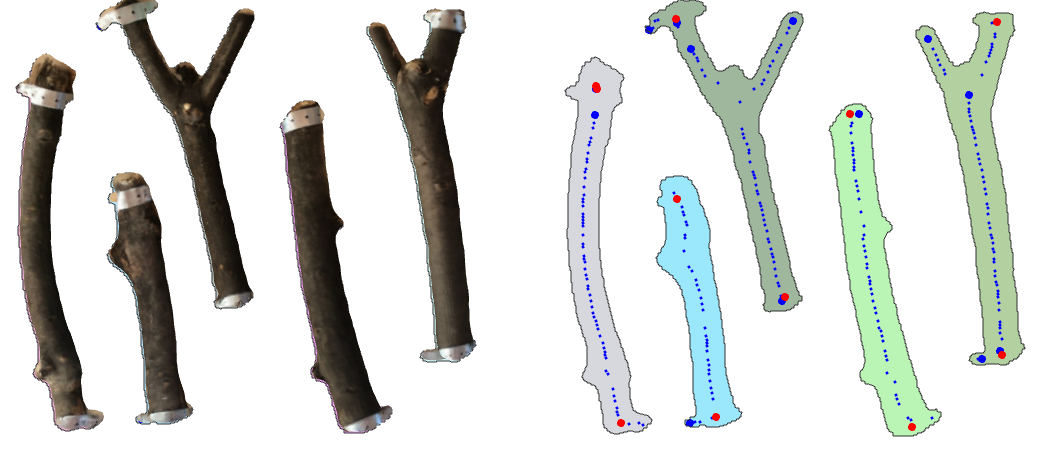
\includegraphics[width = 0.4\paperwidth]{images/importer/importer.png}
  \caption{An interface of \textit{Branch Importer}. Left: a top ortho-view image of textured mesh model. Right: Extracted skeletons are shown with blue dots. The beginning of skeletons is shown bigger dots, and the red dots are invalid points defined by a user. }
  \label{fig:skeleton}
\end{figure}


\subsection{Fabrication}
\label{sec:fabrication}
After a design is selected for fabrication, the validity of the design is further inspected by a high-resolution model.
The \textit{G-Code Generator} displays joineries and milling paths on scanned orientations.
In case joineries are invalid with the high-resolution model, a layout can be easily modified with simple mouse inputs (see Figure \ref{fig:gcode_gen}).
Users can also change milling parameters such as offset ratio for the side cuts, milling bit diameter, depth of joineries, cutting speed, moving height and so forth.
After confirming the fabrication settings and milling paths, it generates G-Code.\\

Some fabrication factors such as invalid points due to metal fixtures and flipped (further described in Seciton \ref{sec:joint}) are already considered by \textit{Branch Importer} and the game system respectively.
In this section, we describe the process of joinery generation.
Each joinery's geometry is parametrically modeled with two planar surfaces on the sides of branches (side cuts) and one planar top surface (center cuts) (see Figure \ref{fig:joint_geometry}.2).
Side cuts have wedged corners for smooth assembly process.
The geometry creates rigid joints with irregularly shaped sections of branches.\\

\begin{figure}[ht]
  \begin{center}
    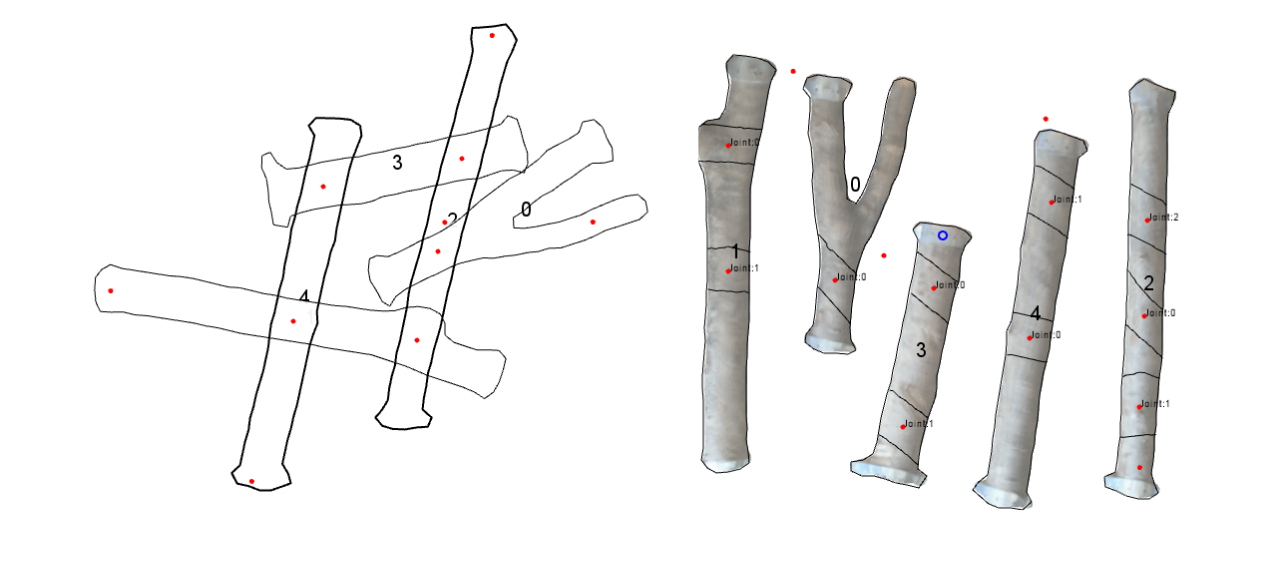
\includegraphics[width = 0.4\paperwidth]{images/system/joint_generator_2.png}
    \caption{Interface of \textit{G-Code Generator}. Left: a layout defined by a user. The calculated joineries are displayed. Right: an original orientation of a scanned plate with joineries. }
    \label{fig:gcode_gen}
  \end{center}
\end{figure}

Similar to the joint searching process with skeletons, the \textit{G-Code Generator} searches a set of four closest points from high-resolution contours, expecting that every intersected contour has four curves.
After finding the four closest points, it trims two curves from each contour of branch. (two from intersecting branch and two from intersected branch) at each joint.
The trimmed contours are transformed to the original scanned orientation and used for generating milling paths.
Two curves from an intersected branch are used for generating side cuts milling paths, which are inwardly offset paths of the original branch contours.
Height of center cuts is half of branch diameter.
The diameter as the joint is calculated with the contour.
We compare this value with actual height from the stored point cloud.
In case of uder-cuts, the system detects different values and adjust the center cuts according to the recalculated diameter.

\begin{figure}[H]
  \begin{center}
    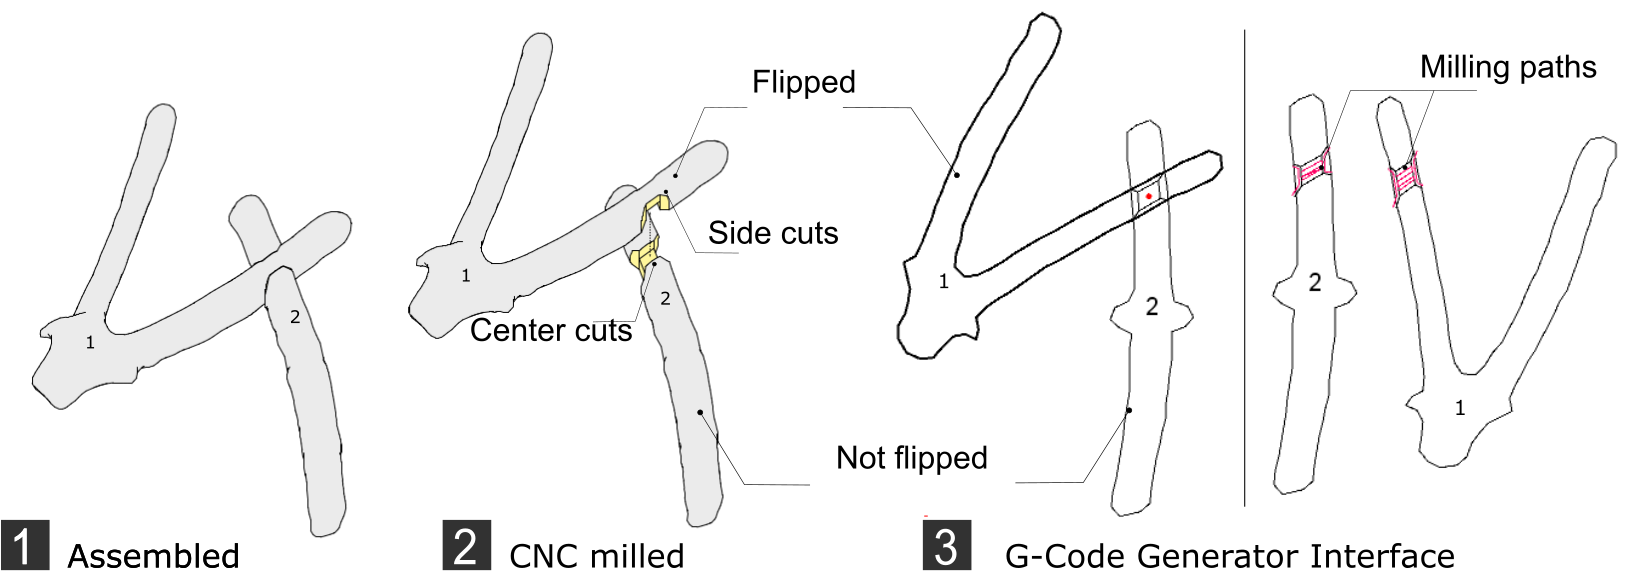
\includegraphics[width = 0.4\paperwidth]{images/system/joint_milling_diagram_4.png}
    \caption{An example of intersected pair: 1. an assembled pair of branches. 2. branches after the center and side cuts are milled 3. left: a layout defined by a user right: the original orientations of branches with generated milling paths with red color.  }
    \label{fig:joint_geometry}
  \end{center}
\end{figure}
